Extending the model to the $n=1$ Landau level modifies the interaction profile: the interaction is effectively multiplied by Laguerre polynomials. While the phase diagram is still expected to partition broadly into valley-polarized and valley-unpolarized regimes, following a similar exchange-driven mechanism, the specific ground-state competition across $(\alpha, W)$ changes.

\section{Anticipated phases}
Across the parameter space, we anticipate the following phase competition:
\begin{itemize}
    \item \textbf{Valley-polarized IQH state (low $W$, small $\alpha$)}: At small inter-valley coupling and low bandwidth, similarly to the LLL case, complete valley polarization is suspected ($\nu = 1 + 0$). Analogously, integer filling in a single valley stabilizes an integer quantum Hall (IQH) state.
    \item \textbf{Paired non-Abelian state ($\alpha = 1$, $W = 0$)}: In the decoupled limit each valley independently hosts a half-filled $n=1$ Landau level ($\nu = \tfrac{1}{2} + \tfrac{1}{2}$). Instead of a composite Fermi liquid, the fermions become unstable to pairing, creating a non-Abelian FTI consisting of two Moore--Read states, $\ket{\mathrm{MR}} \otimes \ket{\overline{\mathrm{MR}}}$ (or $\ket{\mathrm{MR}} \otimes \ket{\mathrm{MR}}$) --- found theoretically in a similar model by Abouelkomsan and Fu~\cite{abouelkomsan2025non}.
    \item \textbf{Depolarization to Fermi liquid (large $W$)}: As the bandwidth $W$ increases, kinetic energy overcomes two-body interactions, eventually forcing a transition to a gapless, unpolarized Fermi liquid (FL).
\end{itemize}

\section{Results for \texorpdfstring{$\nu = 1$}{nu=1} of 1LL (\texorpdfstring{$\nu = 3$}{nu=3} overall)}

Since the Moore--Read state is known to be influenced by the anisotropy of the real-space cluster on which it is defined, tilted boundary conditions were used to stabilize it. To detect the characteristic dependence of the ground-state degeneracy on the fermion-number parity, systems with $N_\phi = 12$ and $N_\phi = 10$ per valley were studied at half filling ($N_e = 12$ and $N_e = 10$, respectively).

\begin{figure}[htbp]
    \centering
    \begin{subfigure}[b]{0.48\textwidth}
        \centering
        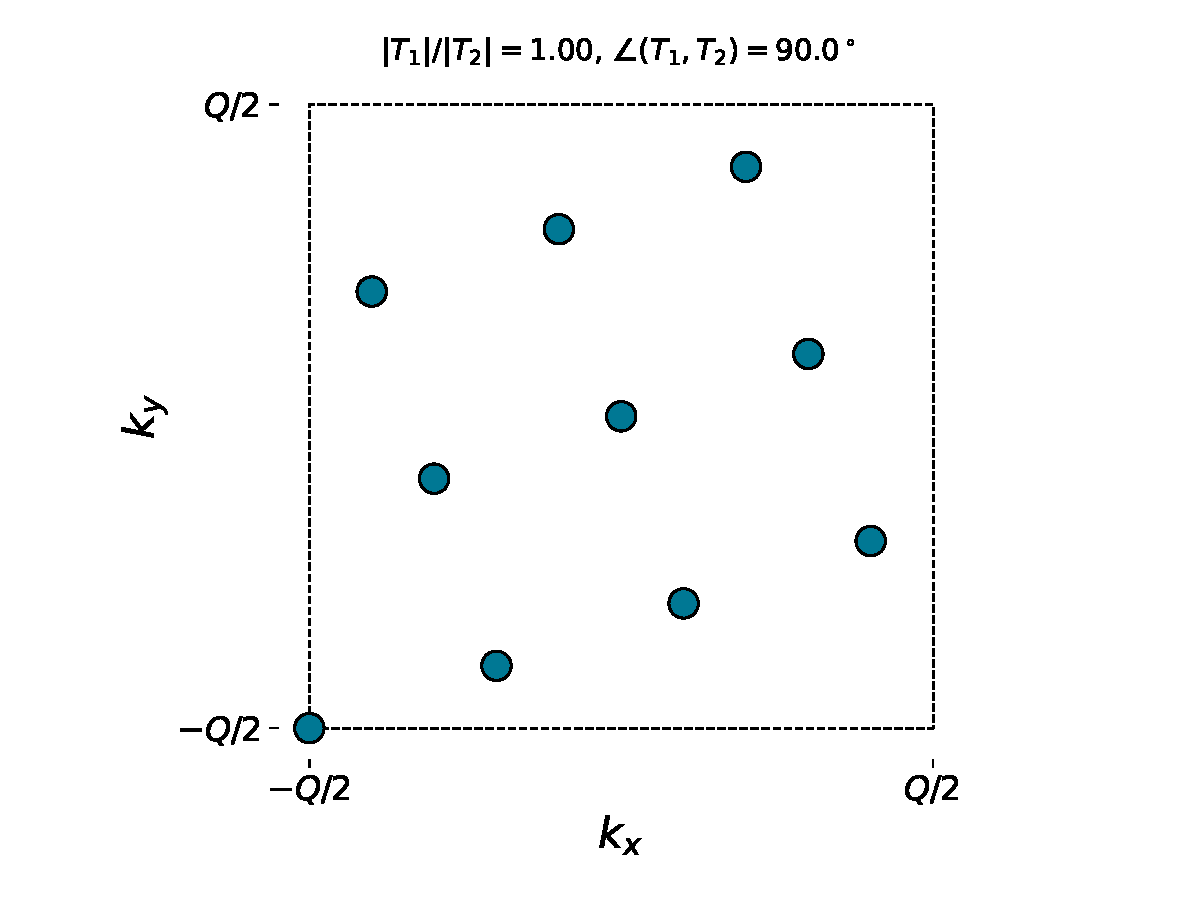
\includegraphics[width=\linewidth]{plots/bz_sampling_tilted_10_ratio=1.000_90.0deg.pdf}
        \caption{$N_\phi = 10$}\label{fig:bz_sampling_10}
    \end{subfigure}
    \begin{subfigure}[b]{0.48\textwidth}
        \centering
        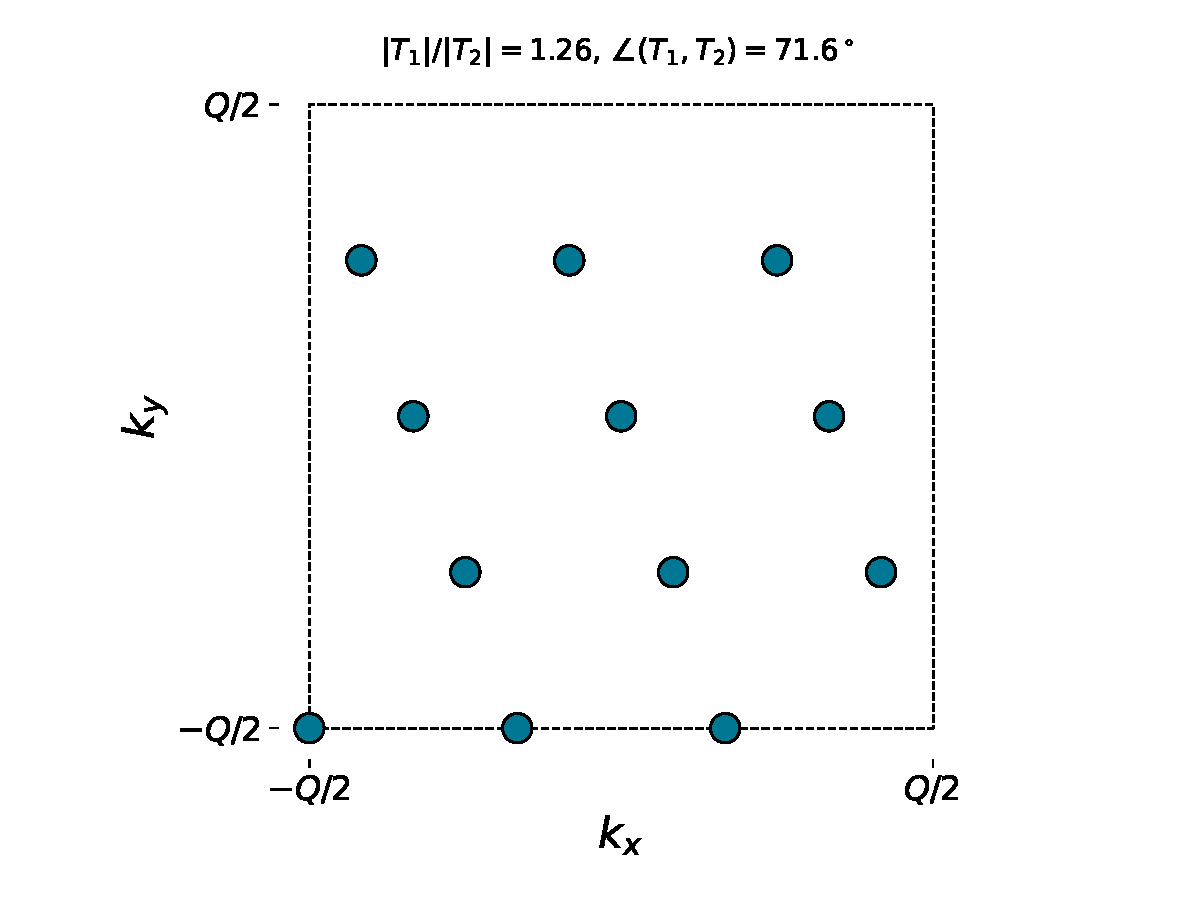
\includegraphics[width=\linewidth]{plots/bz_sampling_tilted_12_ratio=1.265_71.6deg.pdf}
        \caption{$N_\phi = 12$}\label{fig:bz_sampling_12}
    \end{subfigure}
    \caption{BZ sampling for the two system sizes used in the $n=1$ LL calculations, and the properties of the corresponding real-space cluster vectors $T_1$, $T_2$.}
    \label{fig:bz_sampling}
\end{figure}

The tilted lattices used here are shown in Fig.~\ref{fig:bz_sampling}.

\begin{figure}[htbp]
    \centering
    \begin{subfigure}[b]{0.45\textwidth}
        \centering
        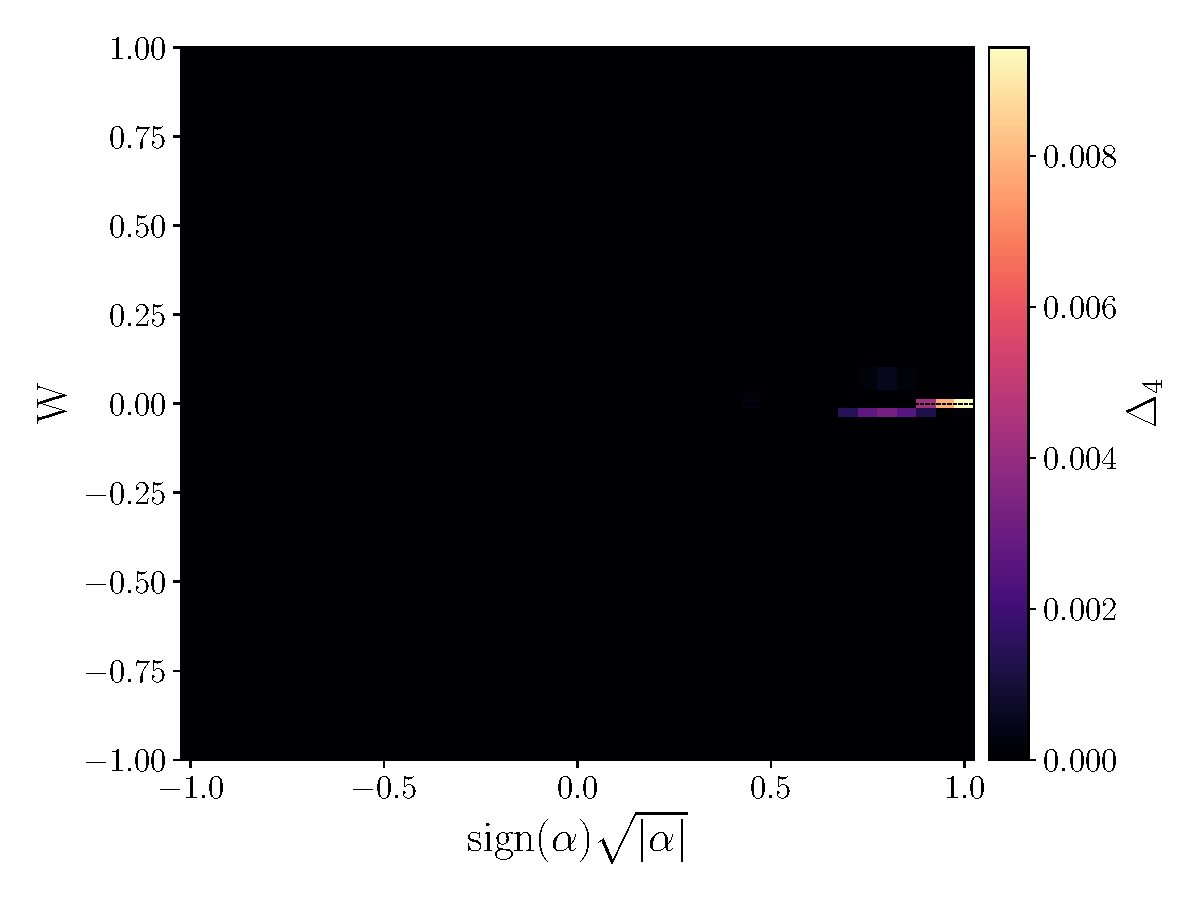
\includegraphics[width=1.0\textwidth]{plots/non_abelian_N10_gap_n4.pdf}
        \subcaption{$\Delta_4$ gap for $N_\phi = 10$ system.}
    \end{subfigure}
    \begin{subfigure}[b]{0.45\textwidth}
        \centering
        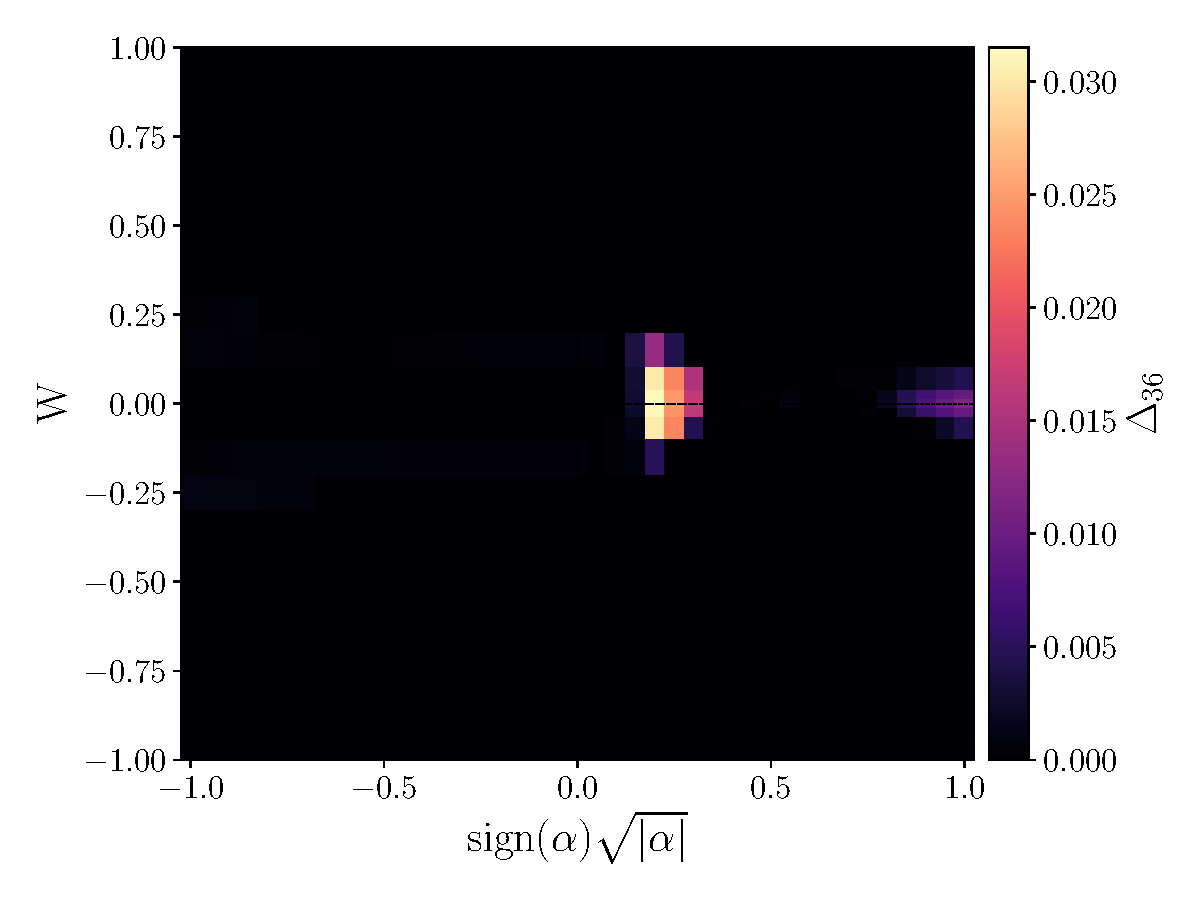
\includegraphics[width=1.0\textwidth]{plots/non_abelian_N12_gap_n36.pdf}
        \subcaption{$\Delta_{36}$ gap for $N_\phi = 12$ system.}\label{fig:non_abelian_gaps_12}
    \end{subfigure}
    \begin{subfigure}[b]{0.45\textwidth}
        \centering
        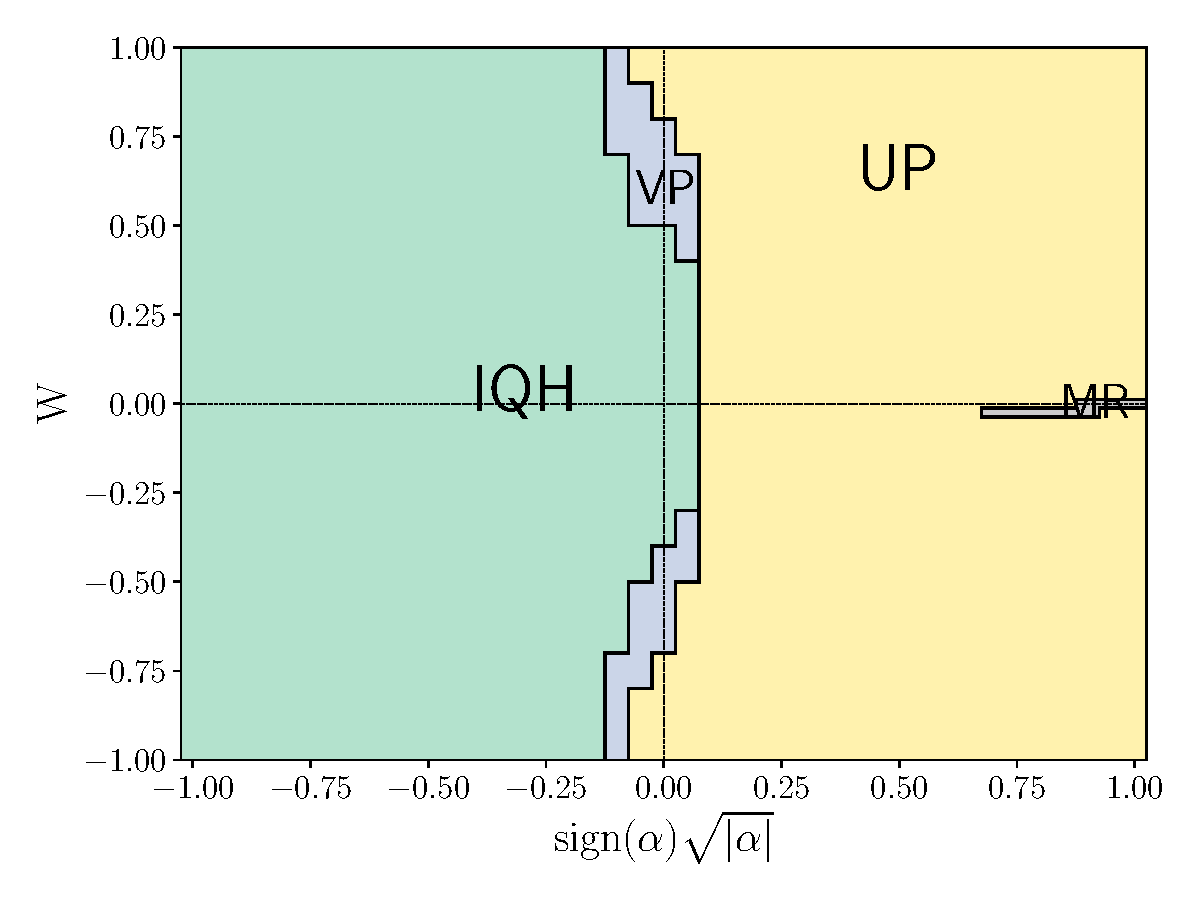
\includegraphics[width=1.0\textwidth]{plots/non_abelian_N10_phase_diagram.pdf}
        \subcaption{Phase diagram for $N_\phi = 10$ system.}
    \end{subfigure}
    \begin{subfigure}[b]{0.45\textwidth}
        \centering
        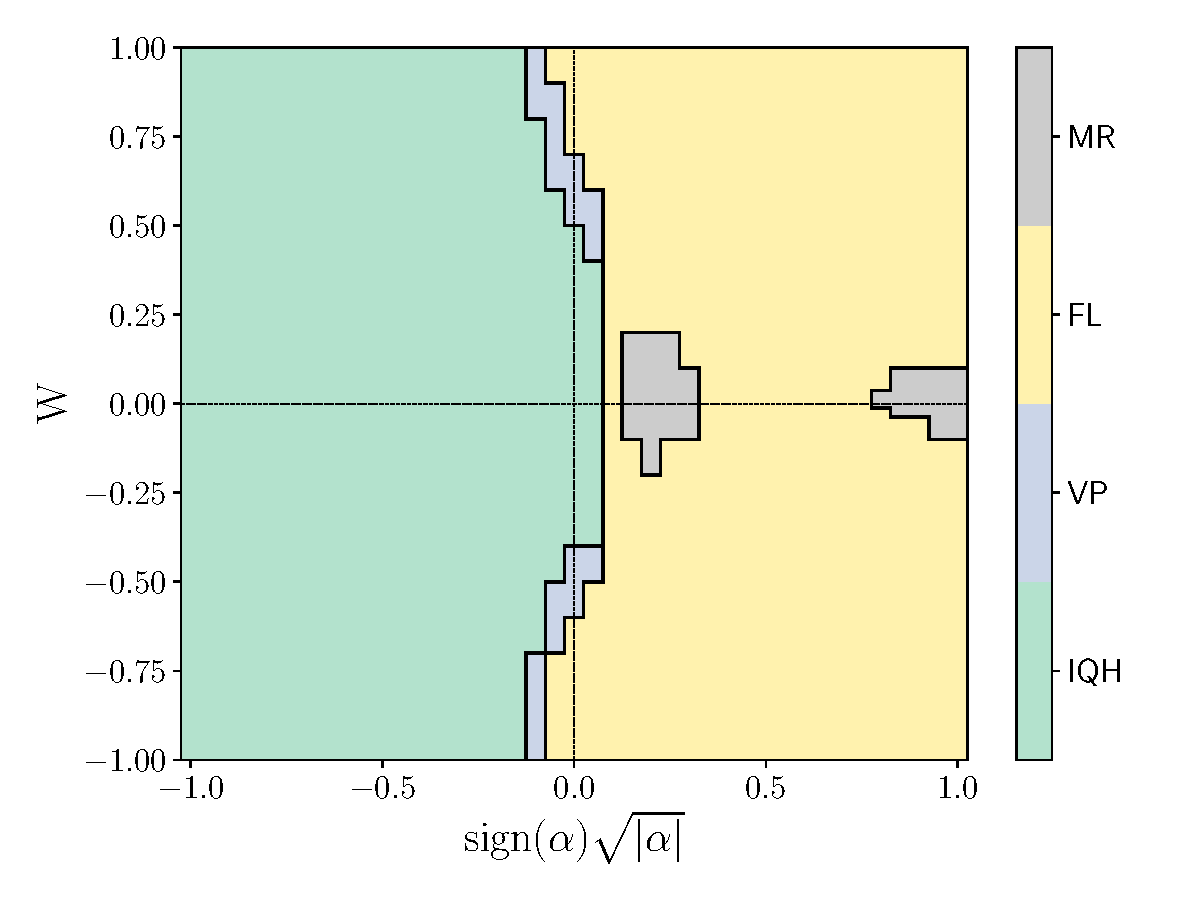
\includegraphics[width=1.0\textwidth]{plots/non_abelian_N12_phase_diagram.pdf}
        \subcaption{Phase diagram for $N_\phi = 12$ system.}
    \end{subfigure}
    \caption{The low-$\alpha$ gapped phase could be just a CDW or something similar --- from a rough look at the flux insertion there is no spectral flow, it seems.}
    \label{fig:non_abelian_gaps}
\end{figure}

Figure~\ref{fig:non_abelian_gaps} shows the $\Delta_4$ and $\Delta_{36}$ gaps for the two system sizes, as well as the schematic phase diagrams. The suspected results are confirmed: at low $\alpha$ and low $W$ the system is in a gapped, valley-polarized phase --- the IQH phase --- and the gap closes at large $W$ as the system transitions to a gapless Fermi liquid, first valley-polarized, then unpolarized. At $\alpha = 1$, $W = 0$, the system is in a gapped, unpolarized phase with 4-fold and 36-fold degeneracy for $N_\phi = 10$ and $N_\phi = 12$ respectively, which is consistent with the expected non-Abelian FTI phase.

\subsection{Problems with the \texorpdfstring{$N_\phi = 12$}{Nphi=12} system}

\begin{figure}[htbp]
    \centering
    \begin{subfigure}[b]{0.48\textwidth}
        \centering
        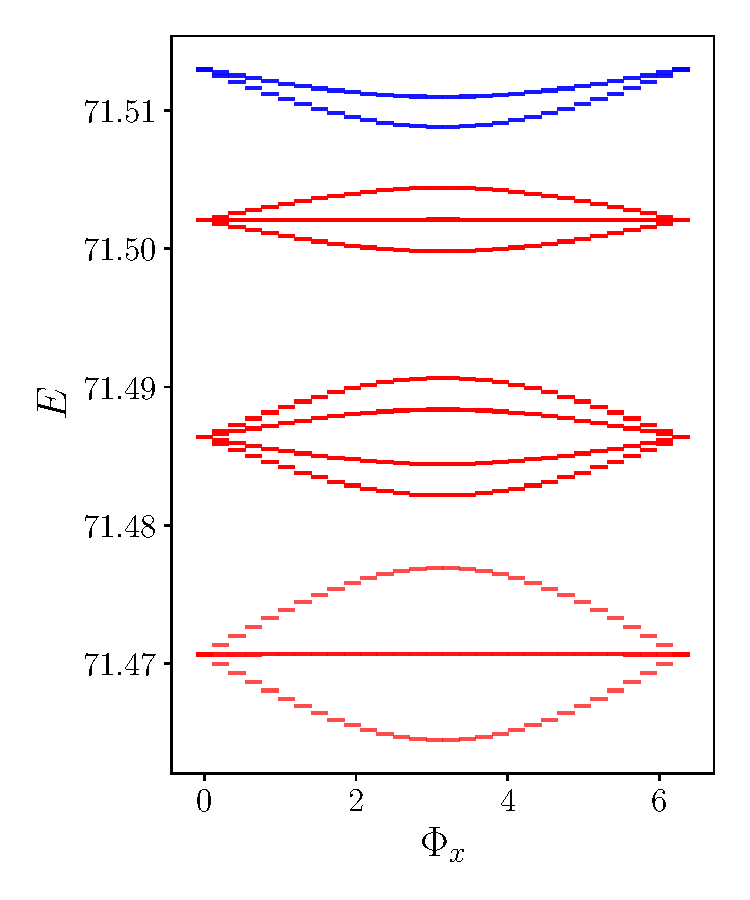
\includegraphics[width=\linewidth]{plots/phase_winding_moore_read_W=0.05_alpha=1.0.pdf}
        \caption{$\alpha = 1.0$}\label{fig:phase_winding_moore_read}
    \end{subfigure}
    \begin{subfigure}[b]{0.48\textwidth}
        \centering
        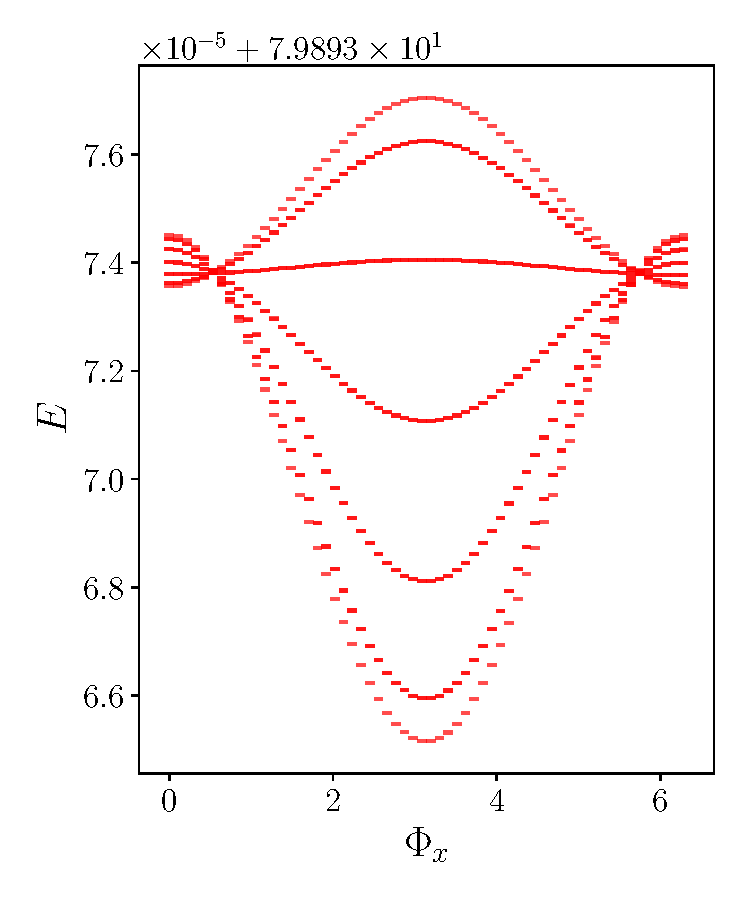
\includegraphics[width=\linewidth]{plots/phase_winding_moore_read_W=0.05_alpha=0.07.pdf}
        \caption{$\alpha = 0.07$}\label{fig:phase_winding_cdw}
    \end{subfigure}
    \caption{Phase winding for $N_\phi = 12$ at $W = 0.05$.}
    \label{fig:phase_winding_1LL}
\end{figure}

Figure~\ref{fig:phase_winding_moore_read} shows a flux-insertion plot for the $N_\phi = 12$ system at $\alpha = 1$, $W = 0.05$. The 36-fold degenerate ground-state manifold is clearly visible, and spectral flow is seen between groups of states in the manifold. However, the gap between the 36-fold degenerate ground-state manifold and the first excited state is in fact smaller than the spread of energies in the ground-state manifold itself. While this is an indication of questionable stability of the phase, it is not a definitive argument against it, as explained below in Sec.~\ref{sec:gap_ratio}.

Second, at the lower end of the unpolarized phase, the size of the $\Delta_{36}$ gap is also quite large (Fig.~\ref{fig:non_abelian_gaps_12}) --- the region is not adiabatically connected to the $\alpha = 1$, $W = 0$ point. Under inspection of the flux insertion (Fig.~\ref{fig:phase_winding_cdw}), it is seen that the spectral flow is not present in this region. The phase is not topological in nature, likely a charge density wave (CDW), and it is not studied further.

\subsection{Discussion of the gap ratio}\label{sec:gap_ratio}

In the literature, due to finite-size effects and dispersion making the ground-state degeneracy only approximate, instead of the direct spectral gap, the ratio of the energy spread $\delta_n$ of the $n$-fold degenerate ground-state manifold to the $\Delta_n$ gap is often considered, with the premise that
\[
    \frac{\delta_n}{\Delta_n} = 0
\]
indicates a perfectly degenerate ground state~\cite{kwan2024could}. A condition of
\[
    \frac{\delta_n}{\Delta_n} < 1
\]
is often used to indicate a good candidate for a topological phase.

Here, I argue that this condition might be too strong when considering a topological insulator made of two decoupled copies of a Chern insulator, $\ket{\mathrm{FTI}} = \ket{\mathrm{FCI}}_- \otimes \ket{\overline{\mathrm{FCI}}}_+$.

Let $E_L$ and $E_H$ be the energies of the lowest and highest states in the $n$-fold degenerate ground-state manifold of the single $\ket{\mathrm{FCI}}_\pm$, and let $E_E$ be the energy of the first excited state. Then $\Delta_n^{\mathrm{FCI\pm}} = E_E^{\mathrm{FCI}} - E_H^{\mathrm{FCI}}$ and $\delta_n^{\mathrm{FCI\pm}} = E_H^{\mathrm{FCI}} - E_L^{\mathrm{FCI}}$, and the ratio of interest is
\[
    \frac{\delta_n^{\mathrm{FCI\pm}}}{\Delta_n^{\mathrm{FCI\pm}}} = \frac{E_H^{\mathrm{FCI}} - E_L^{\mathrm{FCI}}}{E_E^{\mathrm{FCI}} - E_H^{\mathrm{FCI}}}.
\]
The condition imposed for a good topological state is
\[
    \frac{E_H^{\mathrm{FCI}} - E_L^{\mathrm{FCI}}}{E_E^{\mathrm{FCI}} - E_H^{\mathrm{FCI}}} < 1
    \implies
    E_E^{\mathrm{FCI}} - E_H^{\mathrm{FCI}} > E_H^{\mathrm{FCI}} - E_L^{\mathrm{FCI}}
    \implies
    E_E^{\mathrm{FCI}} + E_L^{\mathrm{FCI}} > 2 E_H^{\mathrm{FCI}}.
\]

However, the energies of the $\ket{\mathrm{FTI}}$ are simply the sum of energies of the underlying $\ket{\mathrm{FCI}}_\pm$ states. Thus,
\[
    E_L^{\mathrm{FTI}} = E_L^{\mathrm{FCI}} + E_L^{\mathrm{FCI}}, \qquad
    E_H^{\mathrm{FTI}} = E_H^{\mathrm{FCI}} + E_H^{\mathrm{FCI}}, \qquad
    E_E^{\mathrm{FTI}} = E_L^{\mathrm{FCI}} + E_E^{\mathrm{FCI}},
\]
and
\[
    \Delta_{n^2}^{\mathrm{FTI}} = E_E^{\mathrm{FTI}} - E_H^{\mathrm{FTI}} = E_L^{\mathrm{FCI}} + E_E^{\mathrm{FCI}} - 2 E_H^{\mathrm{FCI}},
\]
which, with the condition imposed above for the FCI, gives simply
\[
    \Delta_{n^2}^{\mathrm{FTI}} > 0.
\]

Thus, the condition for existence of a non-zero gap in the FTI constructed from two decoupled FCI states is equivalent to the condition for a good topological state in the underlying FCI. The condition $\delta_n^{\mathrm{FTI}}/\Delta_n^{\mathrm{FTI}} < 1$ is much stronger than that.

\subsection{Stabilizing the FTI phase --- screening dependence}

Since the non-Abelian FTI phase has a large spread of energies in the ground-state manifold, its stability is tested against the screening parameters $d_{\mathrm{SC}}$ and $l_{\mathrm{RK}}$. For simplicity, the decoupled limit $\alpha = 1$, $W = 0$ is considered, which means each valley can be treated independently --- thus only a single-valley model is considered, where instead of 36-fold degeneracy, a 6-fold degeneracy is expected.

\begin{figure}[htbp]
    \centering
    \begin{subfigure}[b]{0.48\textwidth}
        \centering
        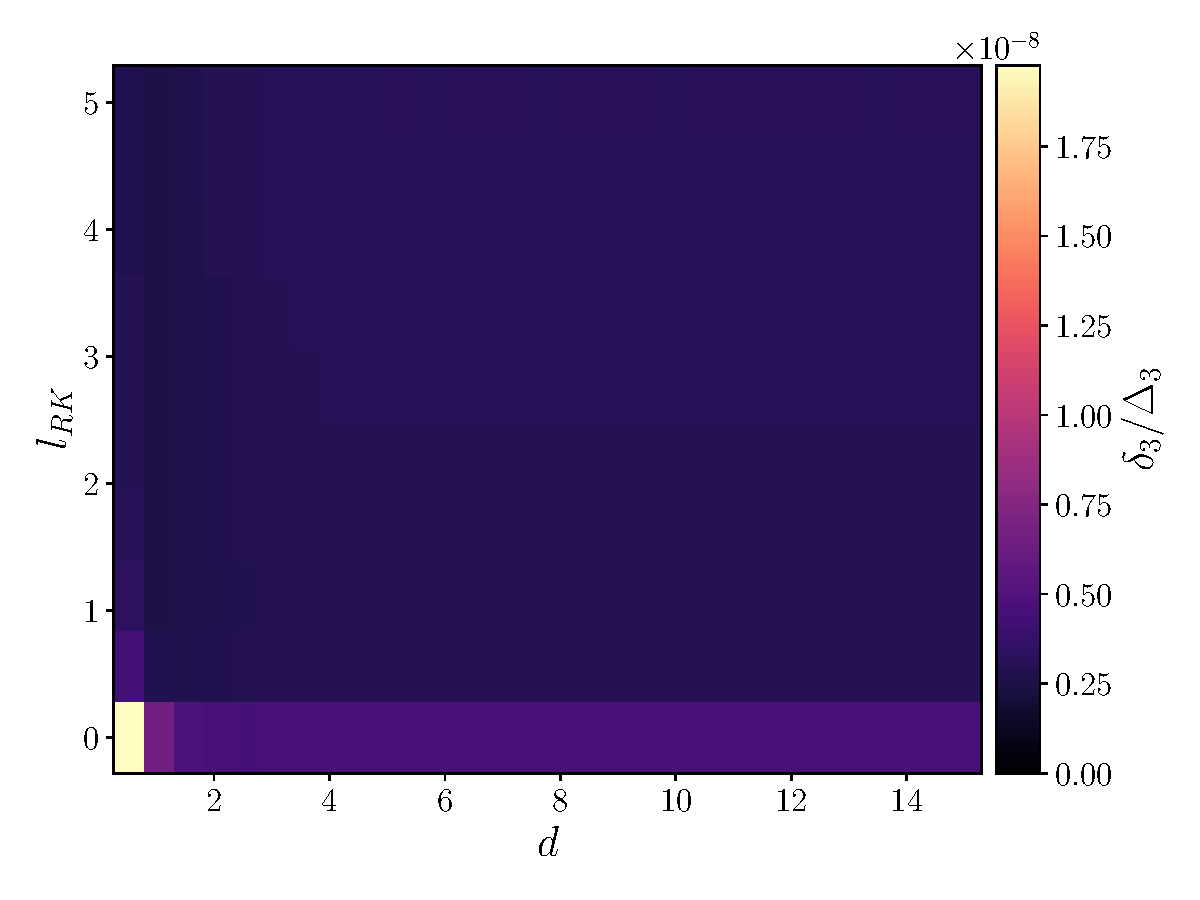
\includegraphics[width=\linewidth]{plots/LLL_stability_n3.pdf}
        \caption{Lowest Landau level}\label{fig:LLL_stability_n3}
    \end{subfigure}
    \begin{subfigure}[b]{0.48\textwidth}
        \centering
        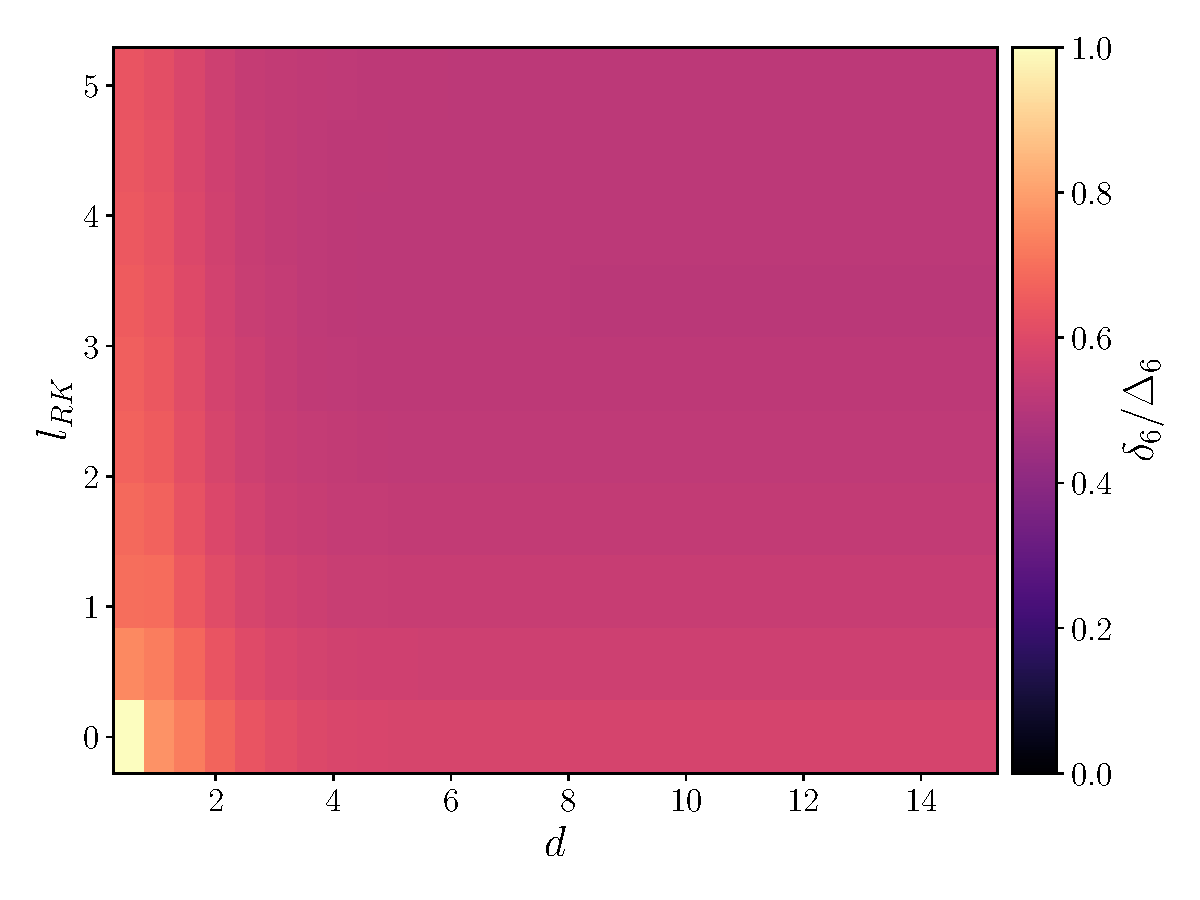
\includegraphics[width=\linewidth]{plots/1LL_stability_n6.pdf}
        \caption{$n=1$ Landau level}\label{fig:1LL_stability_n6}
    \end{subfigure}
    \caption{$\delta_6/\Delta_6$ ratio in one decoupled $\ket{\mathrm{FCI}}$ state corresponding to $W=0$ and $\alpha=1$. Value near zero means good stability.}
    \label{fig:stability_phases}
\end{figure}

In Fig.~\ref{fig:1LL_stability_n6}, the dependence of the $\delta_6/\Delta_6$ ratio on the screening parameters is shown. It is seen that the ratio decreases monotonically with increasing $d_{\mathrm{SC}}$ and $l_{\mathrm{RK}}$. However, comparing with a similar plot for the single-valley $\nu=1/3$ FCI state (Fig.~\ref{fig:LLL_stability_n3}), the ratio is much larger for the $\nu=1/2$ Moore--Read state. While for the lowest Landau level FCI it is consistently close to 0, for the $n=1$ Landau level it does not fall below the $0.5$ threshold. This indicates that the screening of the Coulomb interaction is not sufficient to stabilize the non-Abelian FTI phase.

However, it is important to note that the stability of the FTI phase shown here at the $\alpha=1$ point does not correspond to the stability of the FTI phase in the full $(\alpha, W)$ phase diagram. In Figure~\ref{fig:third_third_screening_alpha_vs_lRK_phase_diagram_b} a maximum of inter--valley coupling stability was seen at $l_{\mathrm{RK}} \neq 0$, while here, the $\delta/\Delta$ ratio decreases monotonically with increasing $l_{\mathrm{RK}}$. This furhter shows the importance of considering the inter-valley interaction.